\documentclass[hyperref={pdfpagelabels=false}]{beamer}
\usepackage{lmodern}
\usepackage{graphicx}
\usepackage{amsmath}
\usetheme{CambridgeUS}

\title{PLEK: a tool for predicting long non-coding RNAs and messenger RNAs based on an improved k-mer scheme}  
\author[Matheus Pimenta]{Matheus Henrique Pimenta Zanon} 
\institute[UTFPR-CP]{\normalsize Universidade Tecnológica Federal do Paraná \\
	Câmpus Cornélio Procópio
} 
\date{19 de Novembro de 2021} 
\begin{document}
	
\begin{frame}
\titlepage
\end{frame} 


\section{PLEK} 
\begin{frame}
\frametitle{PLEK: a tool for predicting long non-coding RNAs and messenger RNAs based on an improved k-mer scheme} 
Paper: \textbf{PLEK: a tool for predicting long non-coding RNAs and messenger RNAs based on an improved k-mer scheme}

Author: Li \textit{et al.}

Journal: BMC Bioinformatics

Date: Sep. 2014

URL: \url{https://doi.org/10.1186/1471-2105-15-311}

\end{frame}

\subsection{Background}
\begin{frame}{Background}
\begin{center}
 \textit{Note: This article is from 2014. From 2014 to the present day a lot of research has been done on the subject.}\pause
\end{center}
\begin{itemize}
 \item  Long non-coding RNAs (lncRNAs, typically $>$200 nt), are of particular interest because they contribute to many important biological processes;\pause
 \item It remains a challenge to distinguish mRNAs from lncRNAs;\pause
 \item LncRNAs show many features similar to mRNAs, such as poly(A) tails, splicing and approximate sequence length.
\end{itemize}
\end{frame}

\begin{frame}
\frametitle{Background}
\begin{itemize}
 \item Several tools, such as CPC and PhyloCSF, have been developed based on known protein databases, intrinsic sequence features and sequence conservation properties.\pause
 \item A tool named Coding-Non-Coding Index (CNCI) was developed. It discriminates coding from non-coding transcripts using intrinsic sequence features.
\end{itemize}

\end{frame}

\begin{frame}
\frametitle{Objective}
\begin{itemize}
 \item A characteristic k-mer based alignment-free tool named PLEK;\pause
\end{itemize}

\vspace{4px}

PLEK takes calibrated k-mer frequencies of a transcript sequence as its computational features. With these features, the support vector machine (SVM) algorithm was used to build a binary classification model to separate lncRNAs from mRNAs.

\end{frame}

\subsection{Implementation}
\begin{frame}
\frametitle{Data description}

Human protein-coding transcripts were downloaded from the \textbf{RefSeq} database (release 60) and human long non-coding transcripts were collected from \textbf{GENCODE v17}. \pause

There were $34,691$ protein-coding transcripts with the length of $>200$ nt in the human \textbf{RefSeq} dataset, and $22,389$ long ($>200$ nt) non-coding transcripts in the human \textbf{GENCODE} dataset.

\end{frame}


\begin{frame}
\frametitle{Improved k-mer scheme}
Approach:  k-mer usage and sliding-windows with a one-nucleotide step-length to analyze each transcript.\pause

A k-mer pattern is a specific string with $k$ nucleotides, each can be $A, C, G$ or $T$. \pause

For $k = 1$ to $5$, had $4 + 16 + 64 + 256 + 1024 = 1,364$ patterns: $4$ one-mer patterns, $16$ two-mer patterns, $64$ three-mer patterns, $256$ four-mer patterns, and $1,024$ five-mer patterns. \pause

Sliding-window of length $k, k = 1,2,...,5$, which slides along the transcript of length $l$ by a step-length of one nucleotide


\begin{align}
 f_i &= \frac{c_i}{s_k}w_k,~k=1,2,3,4,5.~ i=1,2,\dots,1364\\
 s_k &= l-k+1,~k=1,2,3,4,5\\
 w_k &= \frac{1}{4^{5-k}},~k=1,2,3,4,5
\end{align}

\end{frame}

\begin{frame}
\frametitle{Construction of classification model}
To produce a balanced training dataset, we collected all the 22,389 long non-coding transcripts from the \textbf{GENCODE} v17 dataset (labelled as the ``negative” class) and randomly selected 22,389 protein-coding transcripts from the human \textbf{RefSeq} dataset (labelled as the ``positive'' class).

\end{frame}

\begin{frame}
\frametitle{Construction of classification model}
\textbf{Features:} The 1,364 calibrated k-mer usage frequencies of each transcript were regarded as computation features.\pause

\textbf{Scale:} MinMax to range $0$ to $1$, using the $svm-scale$.\pause

\textbf{Classifier:} Support vector machine (SVM) with a radial basis functional kernel, whose variance is gamma, was selected as the binary classifier. \pause

\textbf{Hyper Parameters:}  Optimal C of the SVM and gamma of the kernel were obtained using the grid search. \pause

\textbf{Validation:} 10-fold cross-validation.

\end{frame}

\begin{frame}
\frametitle{Simulation of indel sequencing errors}
PacBio and 454 platforms generate longer reads, which tend to be more easily assembled than short reads. \pause

A tool robust to such errors is desirable to distinguish lncRNAs and mRNAs, and facilitates annotation of lncRNAs and mRNAs of a species without whole-genome sequences. \pause

Simulated 0 to 3 single-base indel sequencing errors per 100 bases (the
error rate p was 0\% to 3\%).

\end{frame}

\begin{frame}
\frametitle{Construction of a real sequencing dataset}

The first dataset was recently released by PacBio and, the second dataset, a HelaS3 cell line transcriptome, was sequenced by a 454 GS FLX Titanium platform.

\end{frame}

\subsection{Results}
\begin{frame}
\frametitle{Different usage frequencies of k-mer strings}
Calculated the calibrated usage frequencies of all the 1,364 k-mer patterns in the positive training dataset (22,389 protein-coding transcripts) and
negative training dataset (22,389 long non-coding transcripts) \pause

Wilcox rank-sum test was used to determine which k-mer pattern usage was significantly different between mRNAs and lncRNAs. \pause

With a significance level of $10^{-6}$, was found that 1,278 patterns were significantly different in their usage

\end{frame}

\begin{frame}
\frametitle{Performance in cross-species prediction}
\begin{figure}
	\centering
	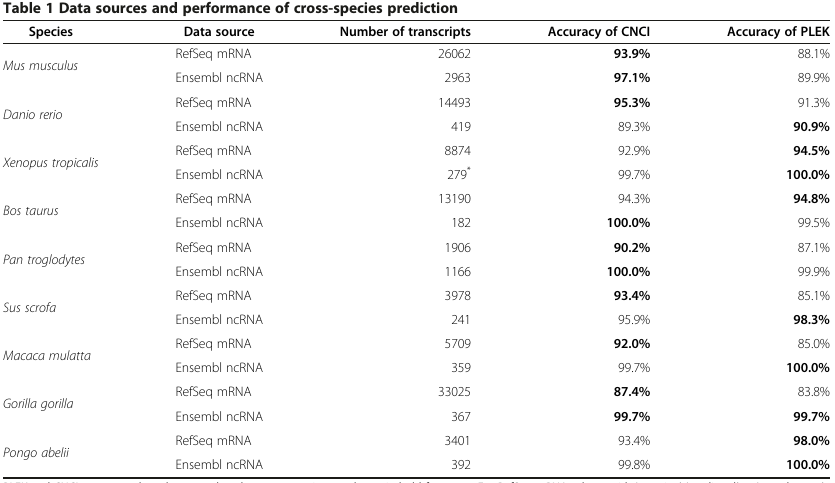
\includegraphics[scale=0.4]{fig1}
	\caption{Data sources and performance of cross-species prediction}
	\label{fig:fig1}
\end{figure}

\end{frame}



\begin{frame}
\frametitle{Robustness to indel sequencing errors}
\begin{figure}
	\centering
	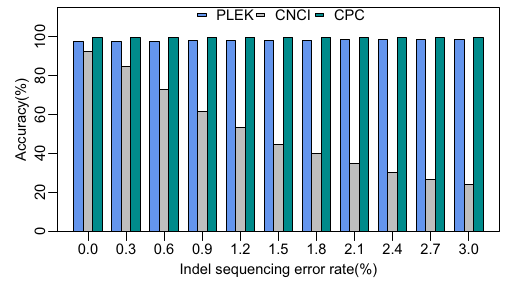
\includegraphics[scale=0.45]{fig2}
	\caption{Comparison of robustness towards indel sequencing errors.}
	\label{fig:fig2}
\end{figure}
\end{frame}

\begin{frame}
\frametitle{Robustness to indel sequencing errors}
\begin{figure}
	\centering
	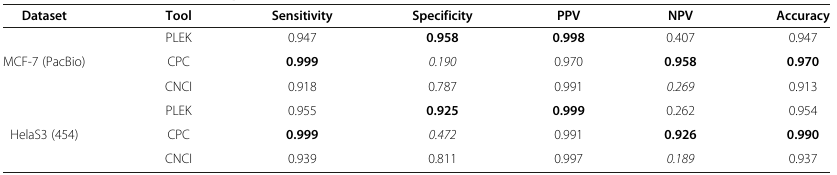
\includegraphics[scale=0.4]{fig3}
	\caption{Performances on transcripts derived from PacBio and 454}
	\label{fig:fig3}
\end{figure}
\end{frame}

\begin{frame}
\frametitle{Performance comparison on mouse datasets}
\begin{figure}
	\centering
	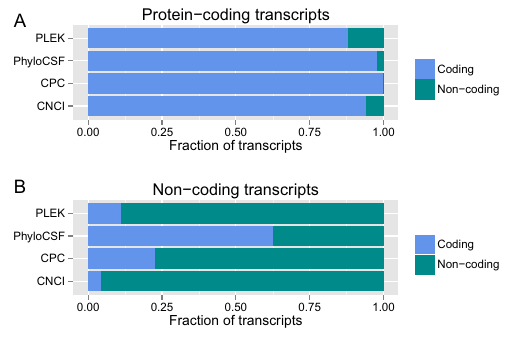
\includegraphics[scale=0.5]{fig4}
	\caption{Results of PLEK, CPC, CNCI and PhyloCSF on mouse datasets.}
	\label{fig:fig4}
\end{figure}
\end{frame}

\begin{frame}
\frametitle{Computational performance}
\begin{figure}
	\centering
	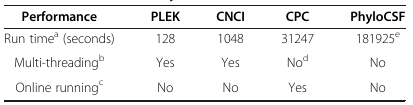
\includegraphics[scale=0.5]{fig5}
	\caption{Comparison of computational performances of PLEK, CNCI, CPC and PhyloCSF}
	\label{fig:fig5}
\end{figure}
\end{frame}

\subsection{Discussion}
\begin{frame}
\frametitle{Discussion}
Prediction accuracy increases with the increasing $k$; however, this is accompanied by an increasing computation load. \pause

\begin{figure}
	\centering
	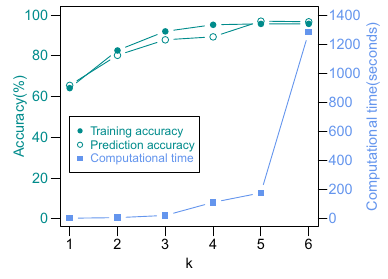
\includegraphics[scale=0.5]{fig6}
	\caption{Performance comparison of various ranges of k.}
	\label{fig:fig5}
\end{figure}
\end{frame}


\subsection{Conclusion}
\begin{frame}
\frametitle{Conclusion}
PLEK is a useful tool for distinguishing protein-coding and non-coding sequences from high-throughput sequencing data of many species without reference genomes. 

\begin{center}
 \textit{Note: This article is from 2014. From 2014 to the present day a lot of research has been done on the subject.}\pause
\end{center}

\end{frame}
\end{document}

